\chapter{Result}\label{Ch:Result}

Figure~\ref{FIG:before_refinement} shows some examples of result before the data refinement steps were applied.
The results seems to contain some face-like objects, but the original faces in the sketch images were not properly translated, resulting in weired colorization in the result. The result of photograph to sketch translation also shows severe artifacts due to the mismatch of locations of faces between datasets.

\begin{figure}[ht]
    \begin{center}
    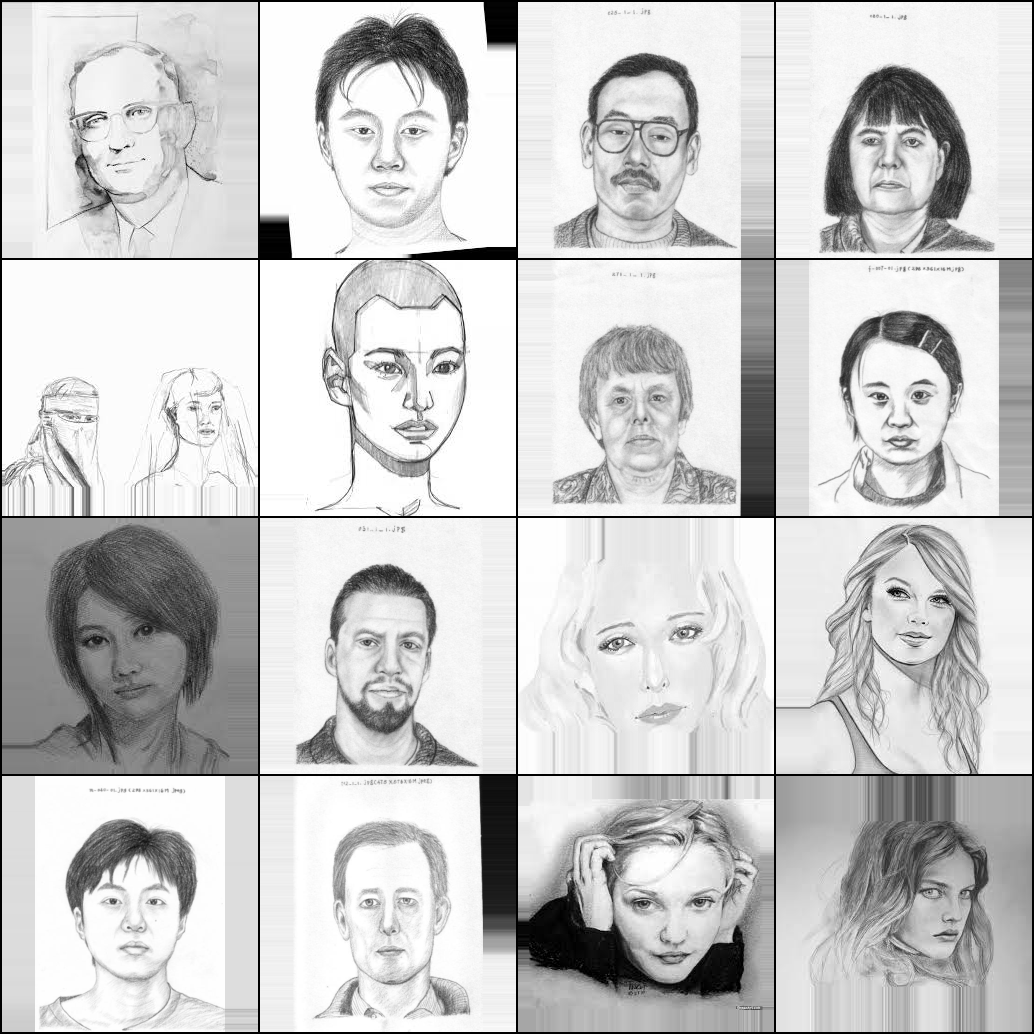
\includegraphics[scale=0.16]{Graphics/ske2pic_origin_before_clean.png}
    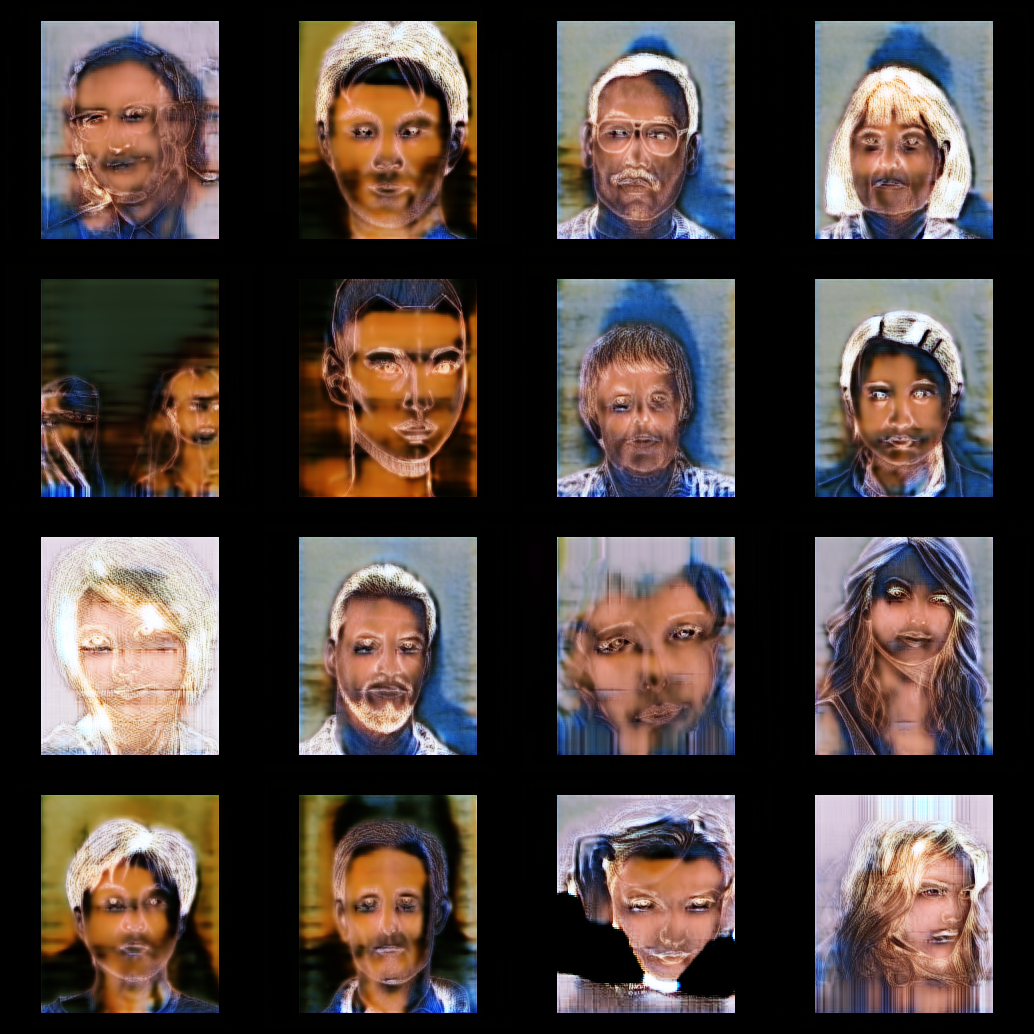
\includegraphics[scale=0.16]{Graphics/ske2pic_result_before_clean.png}

    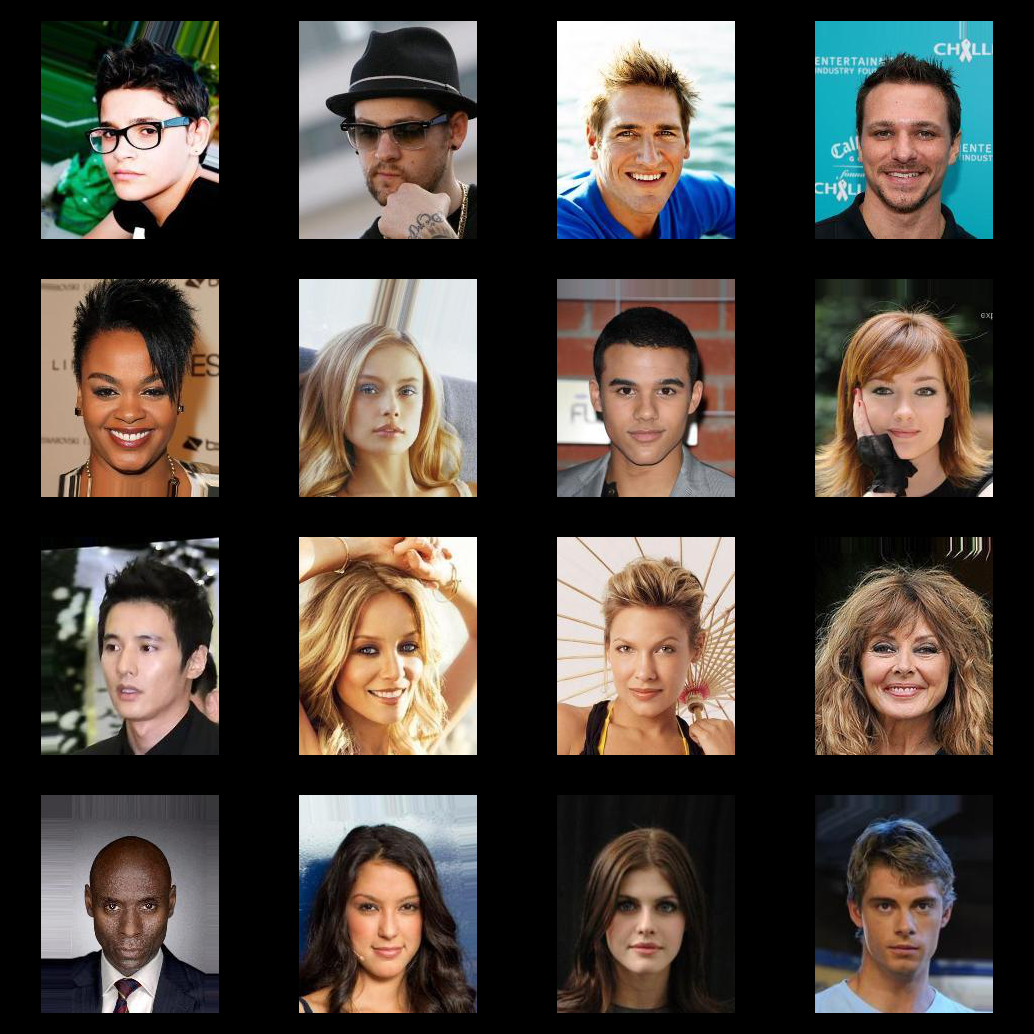
\includegraphics[scale=0.16]{Graphics/pic2ske_origin_before_clean.png}
    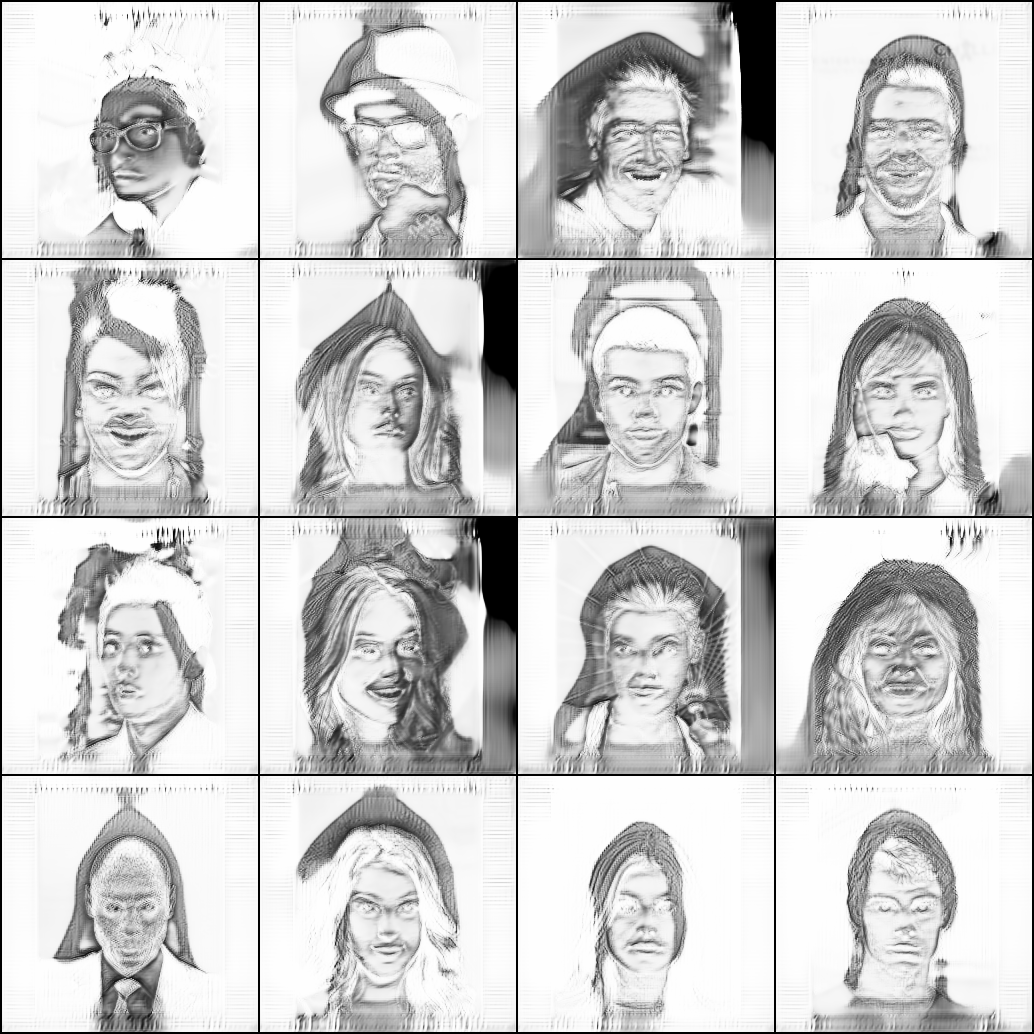
\includegraphics[scale=0.16]{Graphics/pic2ske_result_before_clean.png}
    \end{center}
    \caption{Original input images(left) and result of translations(right) by networks trained before input data is not aligned. Image size is 256 by 256 and model is trained for 64 epochs.}\label{FIG:before_refinement}
\end{figure}


\begin{figure}[ht]
    \begin{center}
    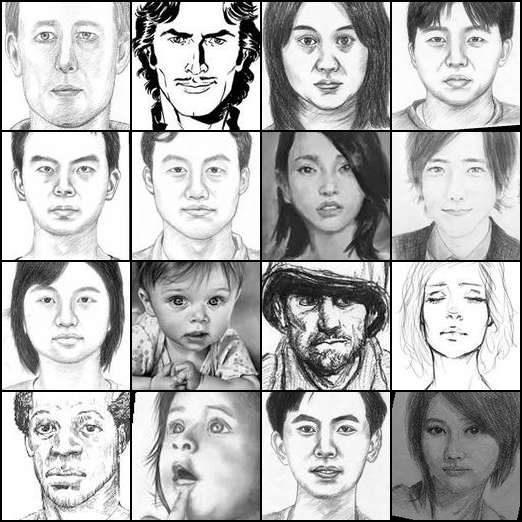
\includegraphics[scale=0.32]{Graphics/smiling_input.png}
    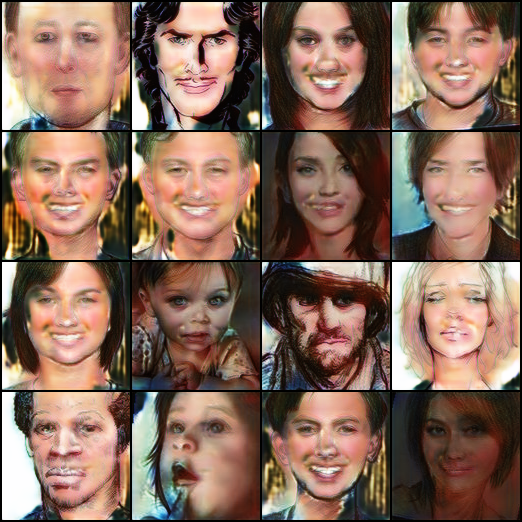
\includegraphics[scale=0.32]{Graphics/smiling_output.png}
    \end{center}
    \caption{Original input images(left) and result of translations(right) by networks trained on datasets after face alignment, but before number of smiling faces was reduced. Image size is 128 by 128 and model is trained for 128 epochs.}\label{FIG:smile}
\end{figure}


\begin{figure}[ht]
    \begin{center}
    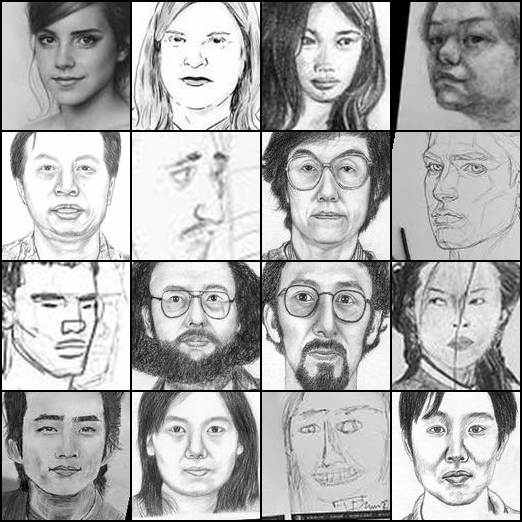
\includegraphics[scale=0.32]{Graphics/ske2pic_origin_final.png}
    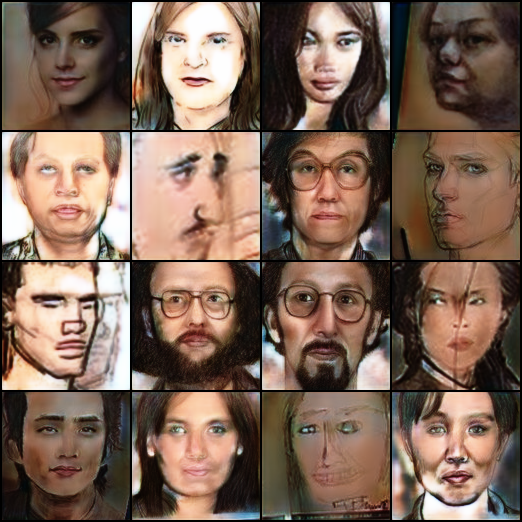
\includegraphics[scale=0.32]{Graphics/ske2pic_result_final.png}

    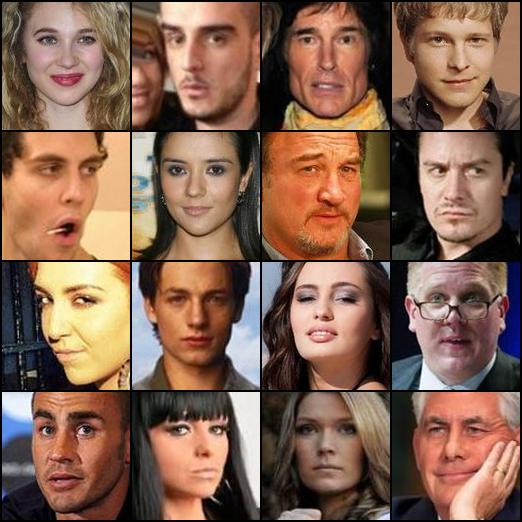
\includegraphics[scale=0.32]{Graphics/pic2ske_origin_final.png}
    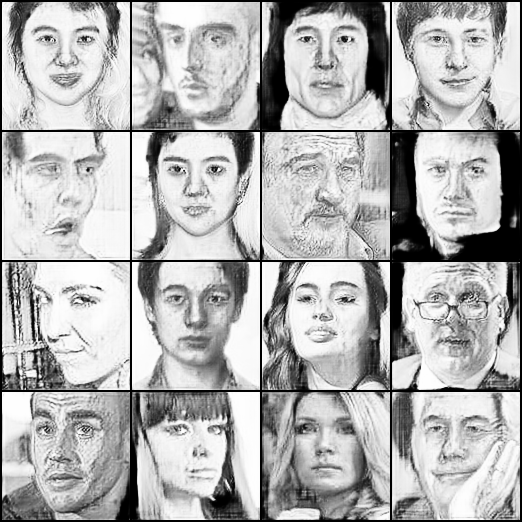
\includegraphics[scale=0.32]{Graphics/pic2ske_result_final.png}
    \end{center}
    \caption{Original input images(left) and result of translations(right) by networks trained on datasets after face alignment and number of smiling faces was reduced. Image size is 128 by 128 and model is trained for 128 epochs.}\label{FIG:final}
\end{figure}



\endinput
